\documentclass[a4paper,12pt]{article}
\usepackage[margin=19mm]{geometry}
\usepackage{amsmath,amssymb,graphicx,xcolor}
\usepackage{fontspec}
\usepackage{xepersian}
\settextfont{XB Roya}
\setlatintextfont{Latin Modern Roman}
\definecolor{ink}{HTML}{173D75}
\graphicspath{{images/}}
\setlength{\parindent}{0pt}
\setlength{\parskip}{5pt}
\linespread{1.12}
\newcommand{\qtitle}[2]{{\Large\bfseries\color{ink} پرسش \lr{#1}: #2}\par}
\newcommand{\answer}{\medskip\textbf{پاسخ یا صورت مورد تأیید و تاریخ:}\par\vspace{18mm}\hrule\medskip}
\begin{document}
{\LARGE\bfseries پرسش‌های ابهام جلسهٔ ۰۹}\par
{\large مدول‌های آزاد، جزوهٔ جبر پیشرفتهٔ دکتر خسروی}\par
شمارهٔ صفحه‌ها، شمارهٔ یک‌مبنای صفحه در فایل پی‌دی‌اف است.
این دو پرسش در تاریخ ۲۵ اکتبر ۲۰۲۶ ثبت شده‌اند و هنوز در انتظار پاسخ‌اند.
\begin{LTR}\small\texttt{sources/lectures/09 Free modules .pdf}\end{LTR}
\medskip\hrule\medskip

\qtitle{L09-Q01}{قید متمایزبودن در تعریف استقلال خطی}
\textbf{وضعیت:} در انتظار پاسخ.\par
\textbf{نشانی منبع:} نسخهٔ \lr{primary}، صفحهٔ ۱، تعریف نخست در بالای صفحه.
\textbf{عبارت منبع:}
\[
\forall x_1,\ldots,x_n\in\mathcal X,\qquad
r_1x_1+\cdots+r_nx_n=0\ \Longrightarrow\ r_1=\cdots=r_n=0.
\]
\begin{center}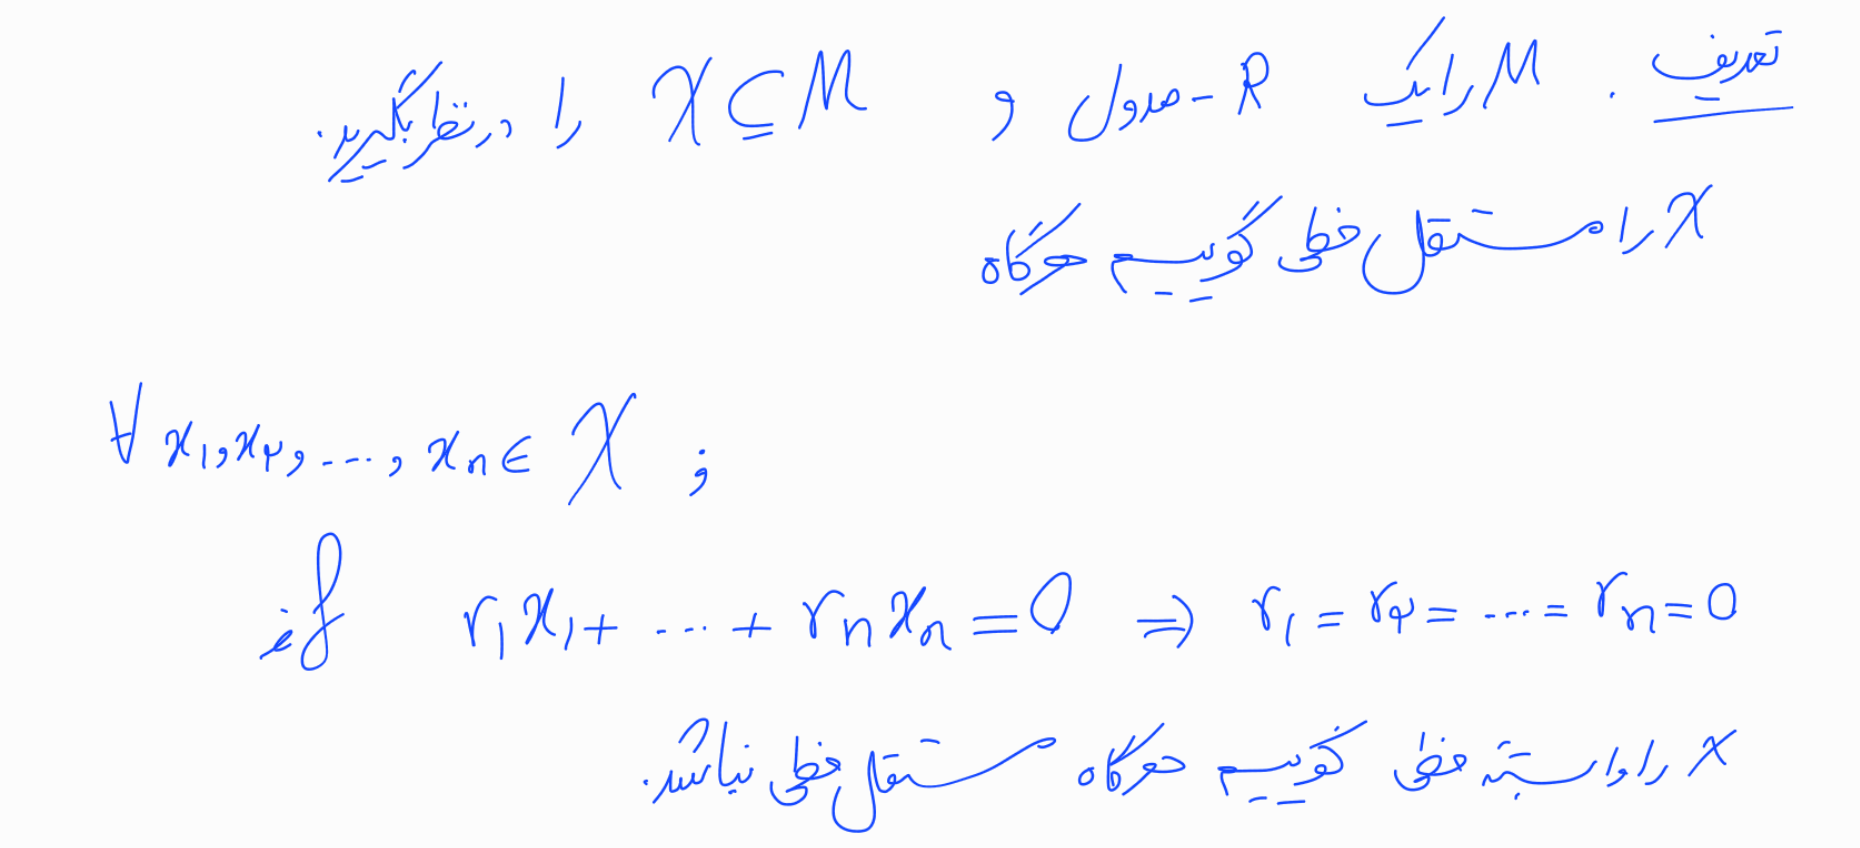
\includegraphics[width=.94\linewidth]{independence.png}\end{center}
\textbf{خوانش‌های ممکن:} شرط برای اعضای دلخواه، با امکان تکرار، یا برای اعضای
دو‌به‌دو متمایزِ $\mathcal X$ منظور شده است. در سطر دست‌نویس قید متمایزبودن
و دامنهٔ ضرایب تصریح نشده است.

\textbf{دلیل پرسش:} با مجازبودن تکرار، انتخاب $x_1=x_2=x$ در یک مدول روی
$\mathbb Z$ رابطهٔ $1x+(-1)x=0$ را می‌دهد و حتی مجموعهٔ تک‌عضویِ ناصفر
نیز مستقل نخواهد بود. این خوانش با نمونه‌های بعدی سازگار نیست.

\textbf{پرسش:} آیا تعریف را با قید «برای هر تعداد متناهی عضو دو‌به‌دو متمایز
$x_1,\ldots,x_n\in\mathcal X$ و هر $r_1,\ldots,r_n\in R$» ثبت کنم؟
\answer
\newpage

\qtitle{L09-Q02}{دامنهٔ $n$ در مثال‌های $\mathbb Z_n$}
\textbf{وضعیت:} در انتظار پاسخ.\par
\textbf{نشانی منبع:} نسخهٔ \lr{primary}، صفحهٔ ۱ پایین صفحه (ناآزادبودن
$\mathbb Z_n$ به‌عنوان $\mathbb Z$-مدول)، و صفحهٔ ۳ میانهٔ صفحه
(نداشتن پایهٔ متناهی و مثال خارج‌قسمت $\mathbb Z/n\mathbb Z$).
\begin{center}
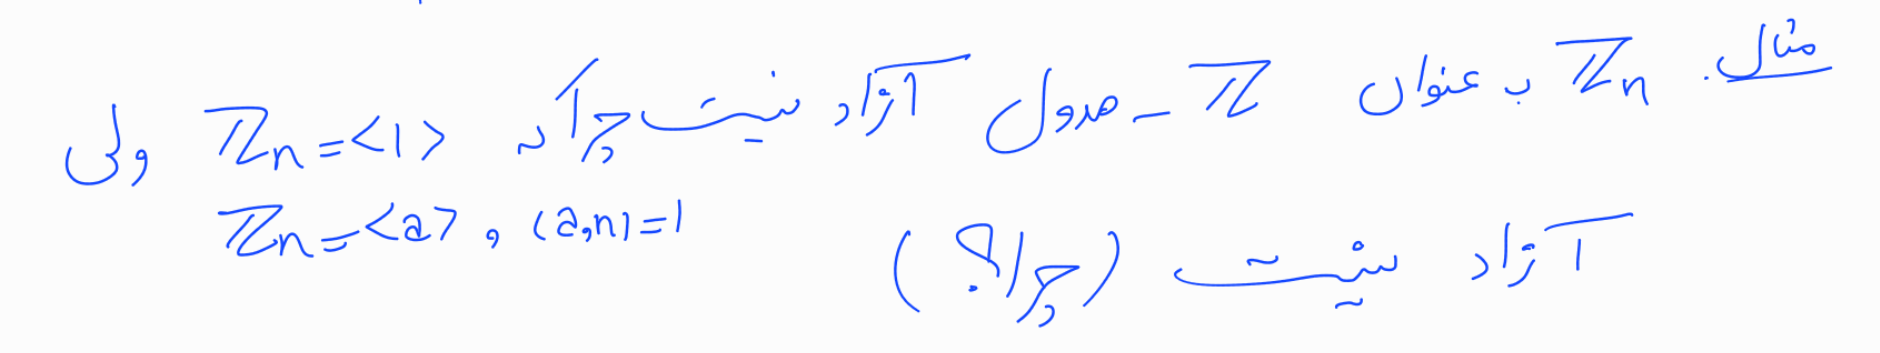
\includegraphics[width=\linewidth]{zn-example.png}\\[4pt]
{\small صفحهٔ ۱}\\[5pt]
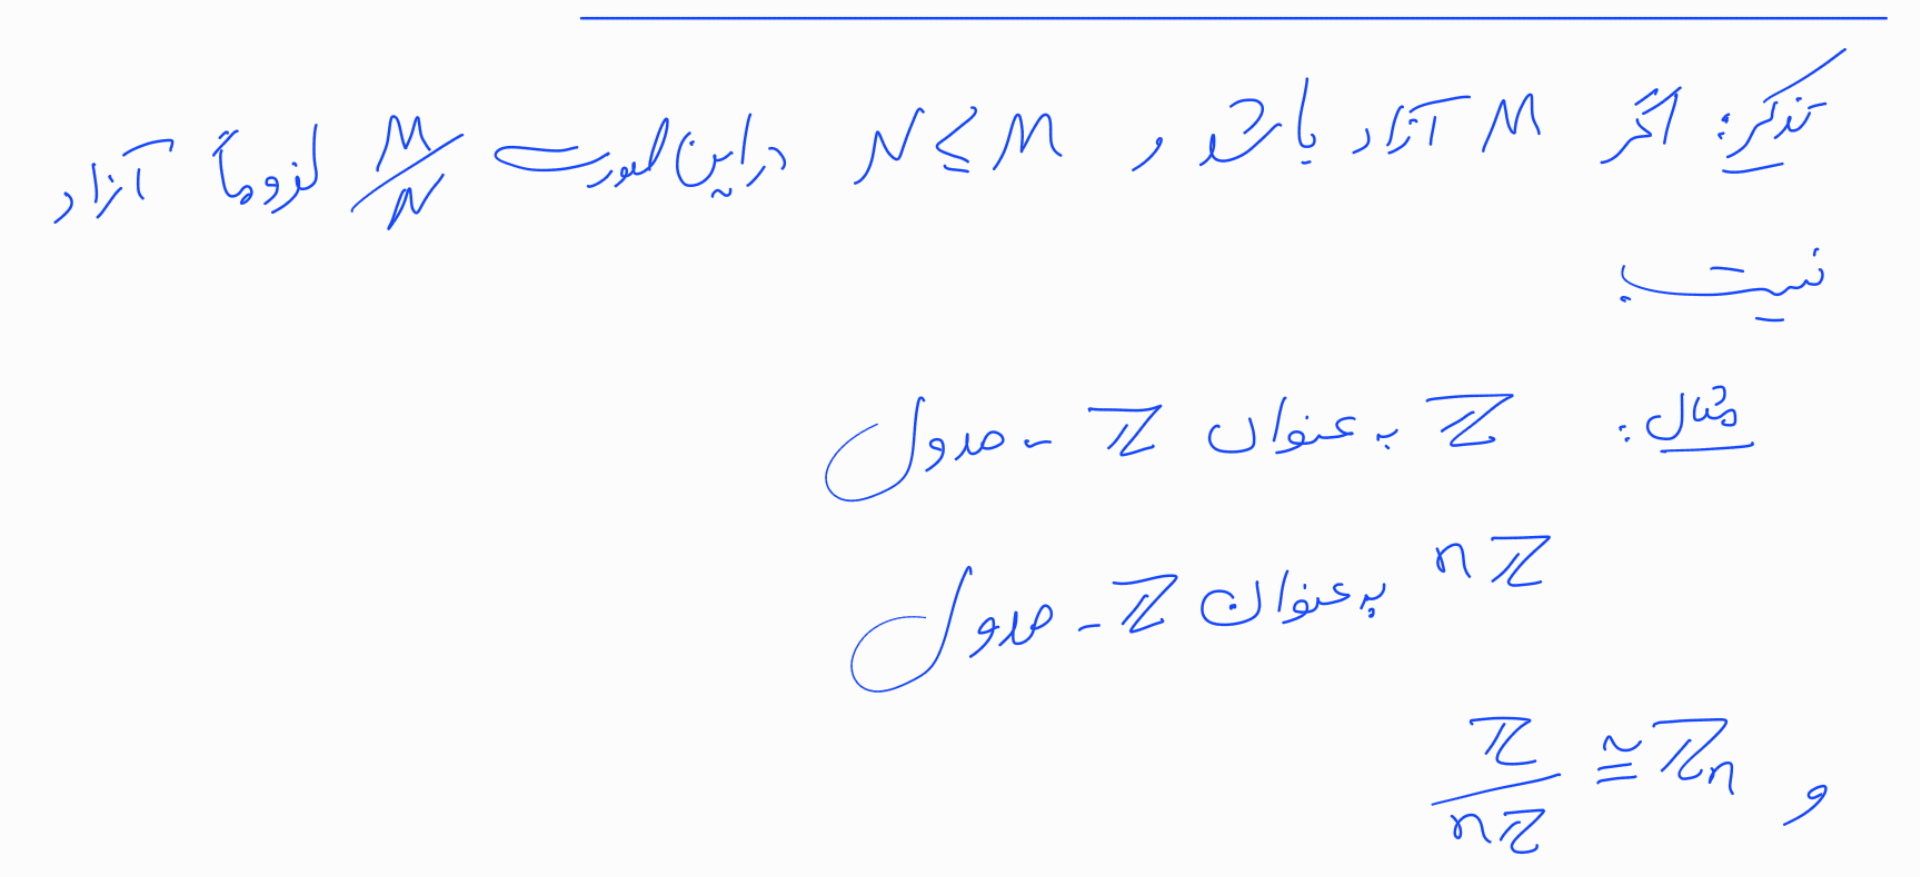
\includegraphics[width=.82\linewidth]{free-quotient.png}\\[3pt]
{\small صفحهٔ ۳، مثال خارج‌قسمت}
\end{center}
\textbf{عبارت منبع:} $\mathbb Z_n$ به‌عنوان $\mathbb Z$-مدول آزاد نیست؛
همچنین $\mathbb Z/n\mathbb Z\cong\mathbb Z_n$ مثال خارج‌قسمت ناآزاد است.
برای $n$ شرطی کنار این مثال‌ها نوشته نشده است.

\textbf{خوانش‌های ممکن:} $n$ عدد صحیح مثبت دلخواه، یا $n\ge2$ است.
\textbf{دلیل پرسش:} برای $n=1$، مدول $\mathbb Z_1=\{0\}$ با پایهٔ تهی
آزاد است؛ خود منبع نیز در صفحهٔ ۱ مدول صفر را آزاد معرفی کرده است.
اگر $n=0$ نیز مجاز باشد، $\mathbb Z/0\mathbb Z\cong\mathbb Z$ آزاد است.

\textbf{پرسش:} آیا در هر سه کاربرد، شرط $n\ge2$ را صریح بنویسم و سایر
مقادیر را از مثال ناآزادبودن کنار بگذارم؟
\answer
\end{document}
